\chapter{緒言}

\section{背景}
\label{section:background}

% エンターテイメントを超えたXRの活用もある
Virtual Reality (VR) や Augmented Reality (AR) などの没入環境の社会実装は昨今急速に
進んでおり,比較的安価なコンシューマ向けのHead Mounted Display (HMD) の登場により,
多くの人が没入環境を体験,利用できるようになった.
没入空間の利用シーンは年々多様化しており,コンシューマ向けのVR/ARマーケットではゲームなど
エンターテイメント向けの利用が目立つが,VRChat\footnote{https://hello.vrchat.com/}や
Horizon World\footnote{https://www.oculus.com/horizon-worlds/}といった
コミュニティに重きを置いた利用も活発になり,コンピュータネットワーク上の新たな世界を指す
メタバースという言葉が流行っている.また没入空間の職業支援や,職業訓練への適用として,
手術\cite{Gallagher2005-gv}や航空宇宙\cite{aerospace},軍事\cite{military},
農業\cite{agriculture}などさまざまな分野での研究が活発であり,
産業界での実際の導入も進んでいることがIDCのレポート\cite{idc-2022}からもわかる.

ここで述べておきたいことは,昨今の没入環境の利用シーンは多様化しており,
様々なコンテキストにおいて没入空間の利用が期待されているという点である.
ここでのコンテキストとは,利用者がどのような目的を持ってどのような作業をしようとしているかを指し,
それは利用時の状況(休日で趣味に時間を使いたいのか,平日で仕事をしたいのかなど)や利用者の職業
などの複雑な組み合わせのもとに生起され,個人ごとの差異があり,個人のなかでもその時々ごとに
連続的に変わってゆくものであるとする.ここで連続的と表現しているのは,ユーザがもつコンテキストは
料理をする,勉強をする,などと離散的に切り替わってゆくものではなく,料理をしながら動画を見る,
料理をしながら一度動画を止めてタイマーを開始する,一度料理をやめてメールを確認する,
と連続的に変化するものであることに注意したいからである.

% 引用する。ref: https://www.sciencedirect.com/science/article/pii/S0747563221004489?casa_token=jobxsigkGQgAAAAA:ZlsQ9qSco-m6yyW-6DJVsP1eifqtqyISE8K_NyA9uzLyYr51nbUa7bbQxzWO0Bh1V6kUEftt5yhh
% 言いたいことをまとめる。 多様化が進んでいて、色々なコンテキストでの利用がある。

\section{問題点}
\label{section:intro:problem}

これから現在の没入環境のパラダイムの問題点を考える前に,これと比較するため2次元の
デスクトップ環境のパラダイムを考察する.
2次元のデスクトップ環境では,1つのスクリーン空間に複数のアプリケーションを立ち上げて使うことが
できる.
アプリケーションは随時開発が可能で,様々な開発元のアプリケーションをダウンロードしたり,
アプリケーションを自分で作成したりして,他の開発元のアプリケーションと同時に組み合わせて利用できる.
アプリケーションの起動や停止も随時可能であるため,ユーザは自分に必要なアプリケーションを
ダウンロードしたり,開発したりしておき,時々のコンテキストに合わせて必要なアプリケーションを
起動して,不要なアプリケーションを停止するということを行っている.
これによって1つのスクリーン空間を柔軟に変化させ,様々なコンテキストに適応させて用いている(図\ref{fig:context-switch}).

\begin{figure}[htbp]
  \centering
  \fbox{
    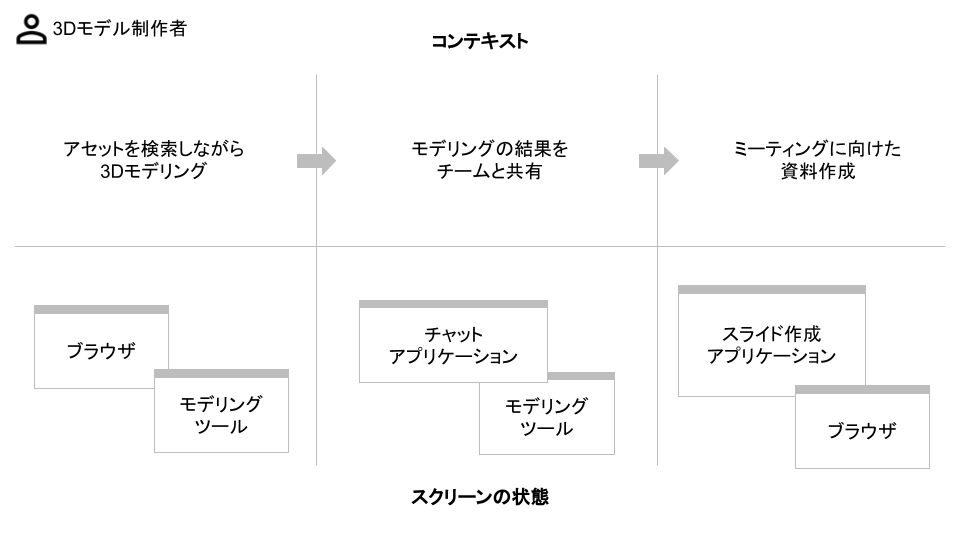
\includegraphics[keepaspectratio, width=0.9\linewidth]{figures/context-switch.png}
  }
  \caption{
    2次元のデスクトップ環境のユーザがコンテキストを変化させてゆく例.
    3Dモデルの制作者を例に,コンテキストを上段の左から右のように変化していくとき,
    3Dモデル制作者は下段のようにそのコンテキストの変化に対応して,アプリケーションを閉じたり,
    新しく開いたりすることでスクリーン空間を柔軟に適応させることができる.
  }
  \label{fig:context-switch}
\end{figure}

以上の点から2次元のデスクトップ環境でのスクリーン空間は不特定のコンテキストに対応可能な,
マルチコンテキストな空間であるといえる.

比較して現在の没入空間のパラダイムでは,基本的に1つのアプリケーションがユーザの視野全体を支配している.
そのためユーザがコンテキストを切り替えるときは,アプリケーションを別のものに切り替え,
全く異なる世界に移動するような形となる(図\ref{fig:switching-app}).
このため,没入環境での3D空間は特定にアプリケーションによって,会議をするといった特定の
コンテキストのために設計されているシングルコンテキストな空間となっている.
没入環境が今後ユーザの普段の生活に溶け込み,継続的に生活や仕事をサポートするようになるためには,
ユーザの連続的に変化し続けるコンテキストに柔軟に対応可能な,新しいパラダイムが必要である.

\begin{figure}[htbp]
  \begin{minipage}[t]{0.55\linewidth}
    \captionsetup[sub]{margin=0.1cm}
    \centering
    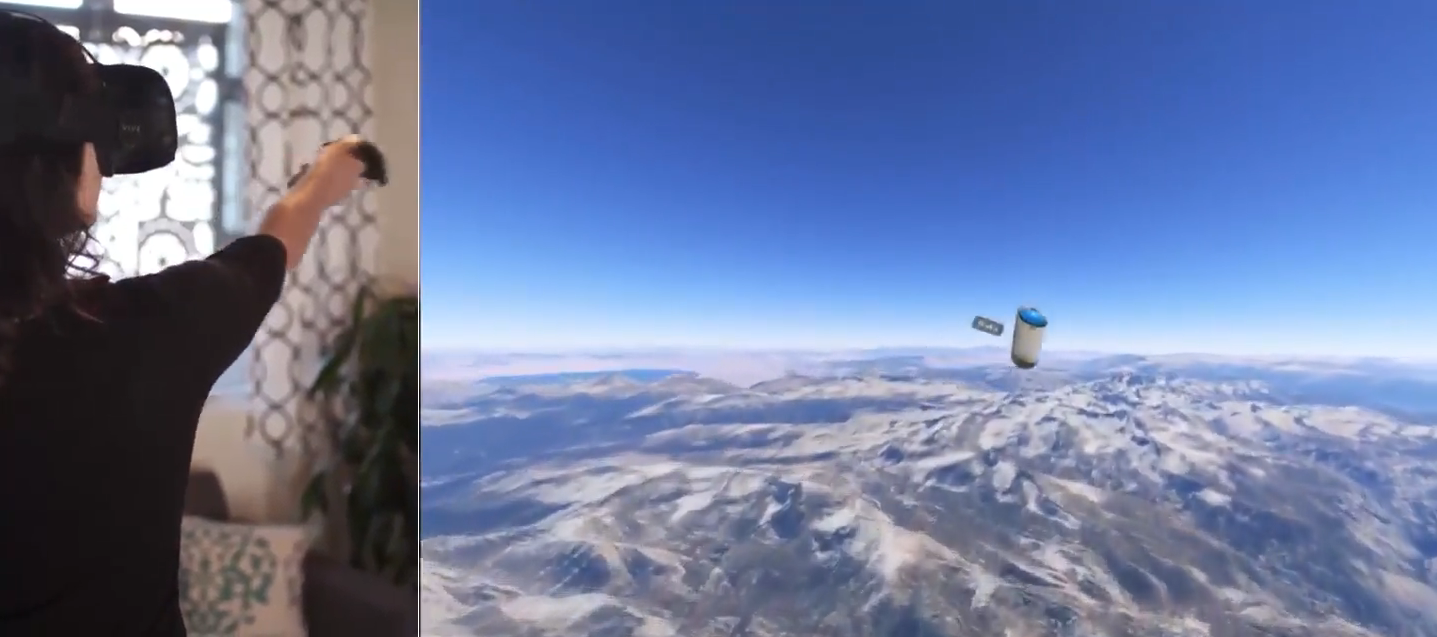
\includegraphics[keepaspectratio, height=1.3in]{figures/google-earth.png}
    \subcaption*{Google.「Google Earth VR」\url{https://arvr.google.com/earth/} (accessed Dec 19, 2022).}
  \end{minipage}
  \begin{minipage}[t]{0.43\linewidth}
    \captionsetup[sub]{margin=0.1cm}
    \centering
    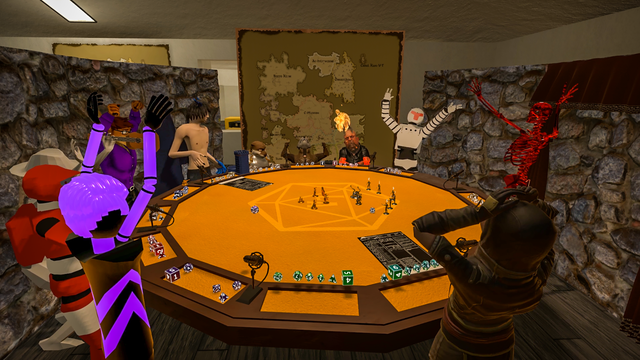
\includegraphics[keepaspectratio, height=1.3in]{figures/vrc.png}
    \subcaption*{VRChat Inc.「PRESS KIT - VRChat」\url{https://hello.vrchat.com/press} (accessed Dec 19, 2022).}
  \end{minipage}
  \caption{
    没入環境でコンテキストを切り替える例.地図を見るというコンテキストから
    大人数でゲームをするというコンテキストへの切り替えを考える.この時ユーザは左図のような
    空間全体を支配した地図アプリケーションの中におり,このアプリケーションを停止し,
    一度ホームの空間に戻る.そこから次は右図のようなソーシャルアプリケーションを起動し,
    そのアプリケーションの世界に入るという流れになる.
  }
  \label{fig:switching-app}
\end{figure}

% ユーザの視野全体を占めている。
% シングルコンテキスト

\section{本研究の目的}

本研究の目的はマルチコンテキストな没入環境の実現を目指し,
その新しいパラダイムの可能性を詳細に検討することである.
その検討が机上の空論とならないために,本研究では実際に動くシステムを実装しており,
現状のエンジニアリング的な制約や,コンピューティングリソースの制約からくる限界にも目を向ける.

% マルチコンテキスト
% より自由な市場の実現
% 実際に動くSystemを実装している。そのデザインを詳細に述べることで、今後のベースラインになることを期待する。

\section{本論文の構成}

本論文では特に,マルチコンテキストな没入空間を実現するためのシステムデザインや,
技術的な課題の解決に関しての研究成果をまとめている.
